\documentclass[a4paper, 12pt]{article}

\usepackage[utf8]{inputenc}
\usepackage[T1]{fontenc}
\usepackage{lmodern}
\usepackage{amsmath, amssymb}
\usepackage{graphicx}
\usepackage{geometry}
\usepackage{hyperref}
\graphicspath{{images}}

\geometry{margin=1in}

\title{Amsterdam}
\author{Lars De Volder}
\date{\today}

\begin{document}

\maketitle

\section{Vervoer}

NMBS International: \url{http://www.b-europe.com/}:
\begin{itemize}
    \item Heen: Brugge 8u58 --- Amsterdam Centraal 12u09 (3u11) €26,20
    \item Terugreis, verschillende opties: ongeveer elk uur een trein rond de €25, 3u reistijd.
\end{itemize}

\section{Verblijf}

Generator Amsterdam: \url{https://www.booking.com/hotel/nl/generator-amsterdam.en-gb.html}\\
\begin{figure}[h]
    \centering
    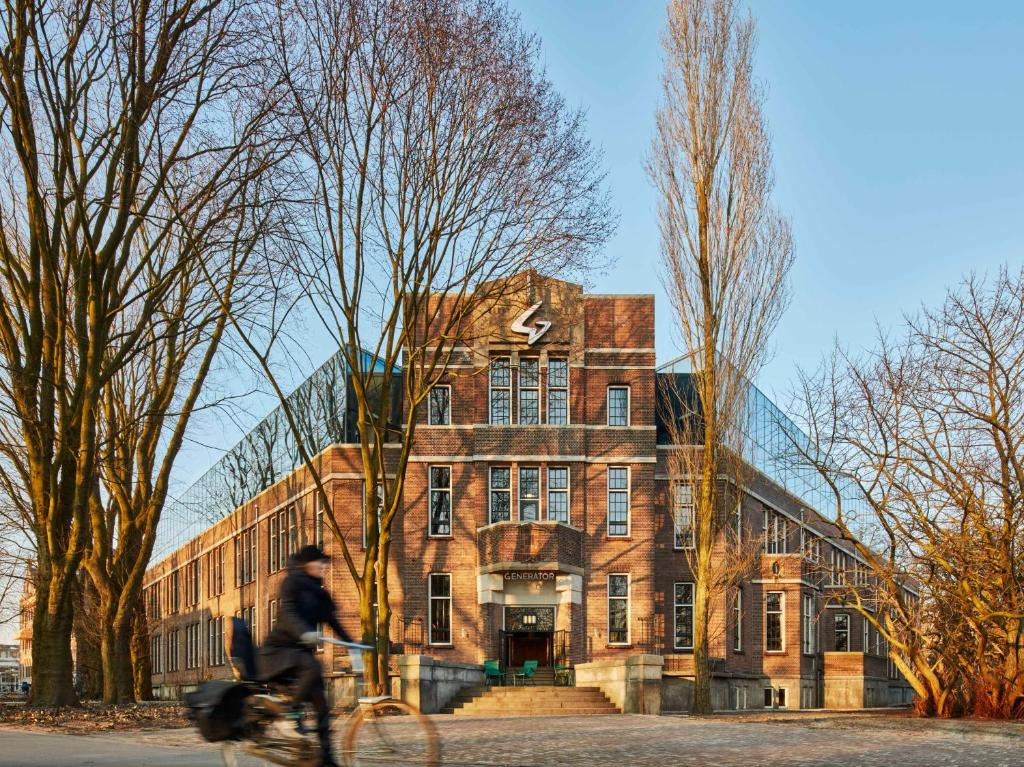
\includegraphics[width=0.5\textwidth]{generator_amsterdam.jpg}\label{fig:generator_amsterdam}
    \caption{Generator Amsterdam}
\end{figure}
4 personen, €90 per nacht. Eigen badkamer.

\subsection{Ligging}
\begin{itemize}
    \item 20 min ov van Amsterdam Centraal
    \item 17 min ov Rijksmuseum en Van Gogh Museum
    \item 34 min ov Anne Frank Huis
\end{itemize}
Eerste ritje zal 10--15 minuten duren, maar eenmaal we in het centrum zijn is alles dichtbij.

\begin{figure}
    \centering
    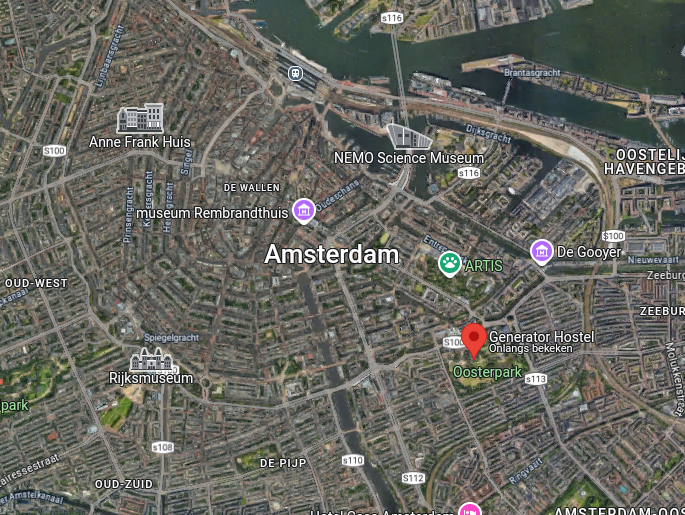
\includegraphics[width=0.5\textwidth]{ligging.png}\label{fig:ligging}
    \caption{Ligging hostel}
\end{figure}

\section{Verplaatsing}

Openbaar vervoer: \url{https://www.gvb.nl/}:
\begin{itemize}
    \item 2 dagen onbeperkt reizen (bus, tram, en metro): €24,00 (\hyperlink{https://www.gvb.nl/reisproducten/toeristen/amsterdam-travel-ticket}{Amsterdam travel ticket})
    \item Per rit betalen: €1,08 + €0,196/km (\hyperlink{https://www.gvb.nl/reisproducten/saldo/saldo}{Saldo}),
     kan ook contactloos met Maestro, Visa, Google Wallet of Apple Pay
\end{itemize}

\section{Activiteiten}

Verschillende dingen worden best vooraf gereserveerd, zoals het Anne Frank Huis.
Deze lijst is niet exhaustief, maar geeft een idee van wat er te doen is.

\subsection{Anne Frank Huis}
\url{https://www.annefrank.org/nl/museum/tickets/}\\
€16,00 per persoon (geen studentenkorting), moet vooraf geboekt worden.\\
Volgens mij een must-see, alhoewel het niet goedkoop is.

\begin{figure}[h]
    \centering
    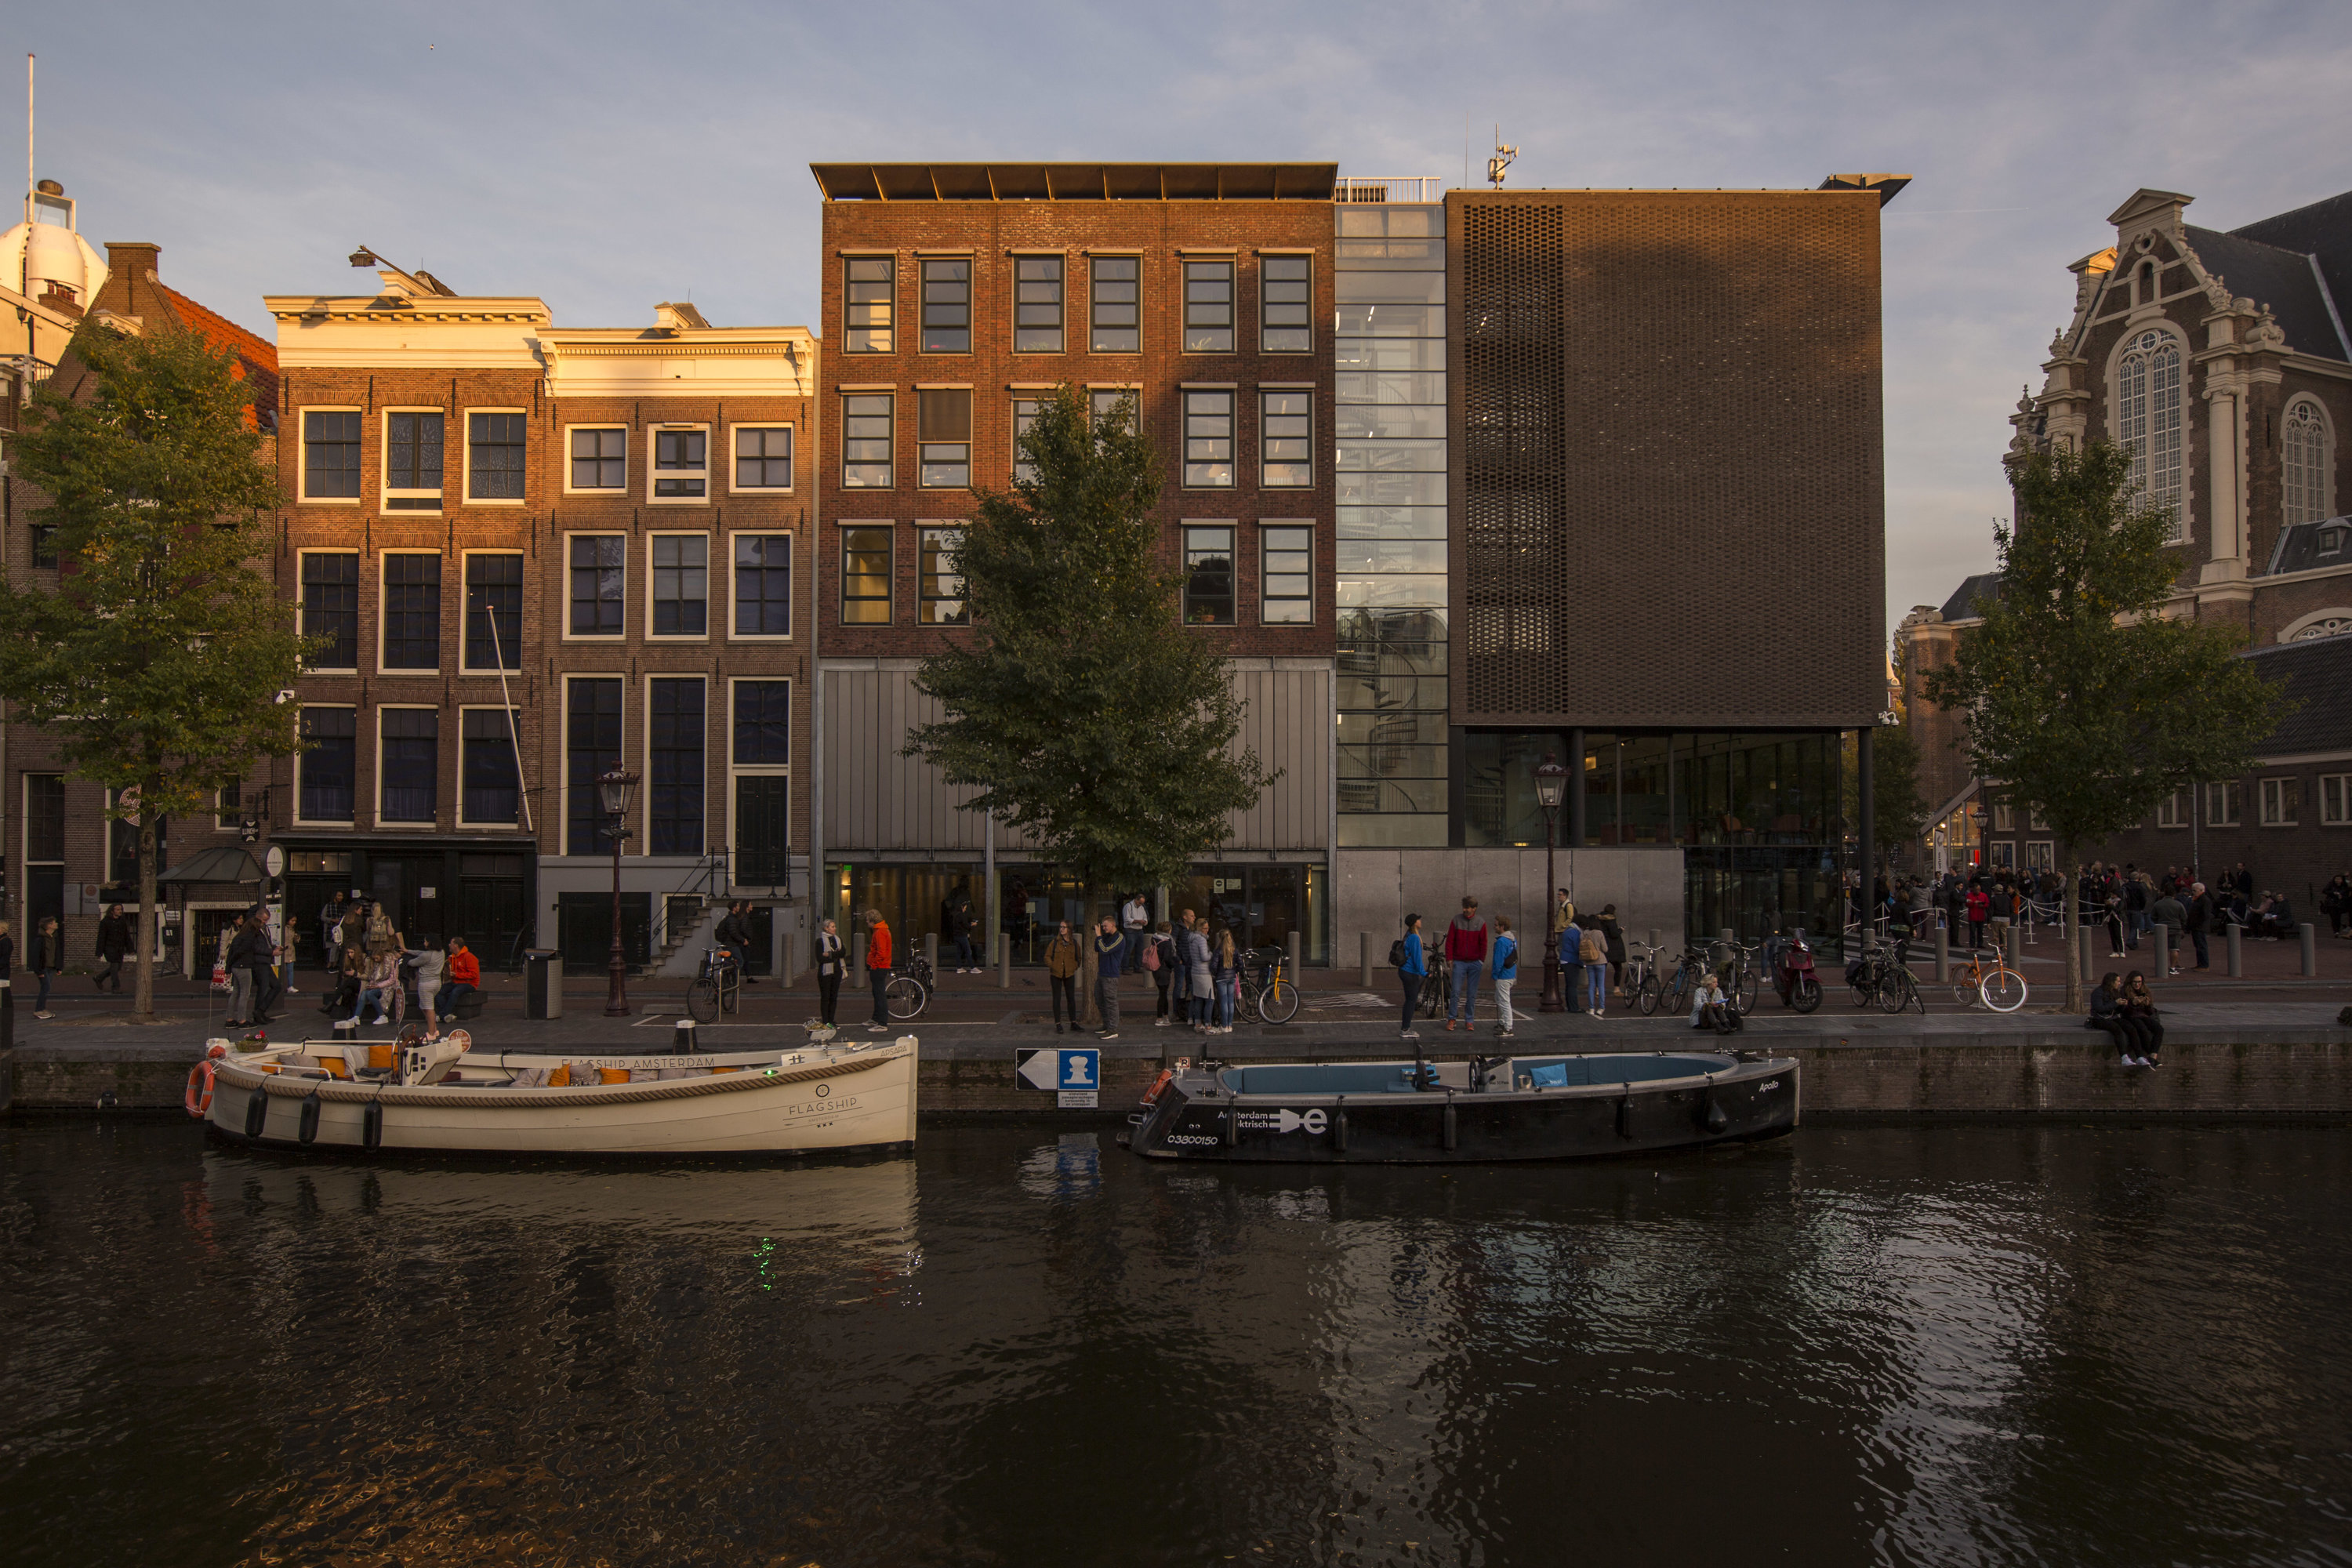
\includegraphics[width=0.5\textwidth]{anne_frank.jpg}\label{fig:anne_frank}
    \caption{Anne Frank Huis}
\end{figure}

\subsection{Van Gogh Museum}
\url{https://www.vangoghmuseum.nl/nl}\\
€11,00 per persoon (studentenkorting), snel uitverkocht.\\
Groot kunstenaar, volgens velen zeker de moeite waard om te bezoeken.

\begin{figure}[h]
    \centering
    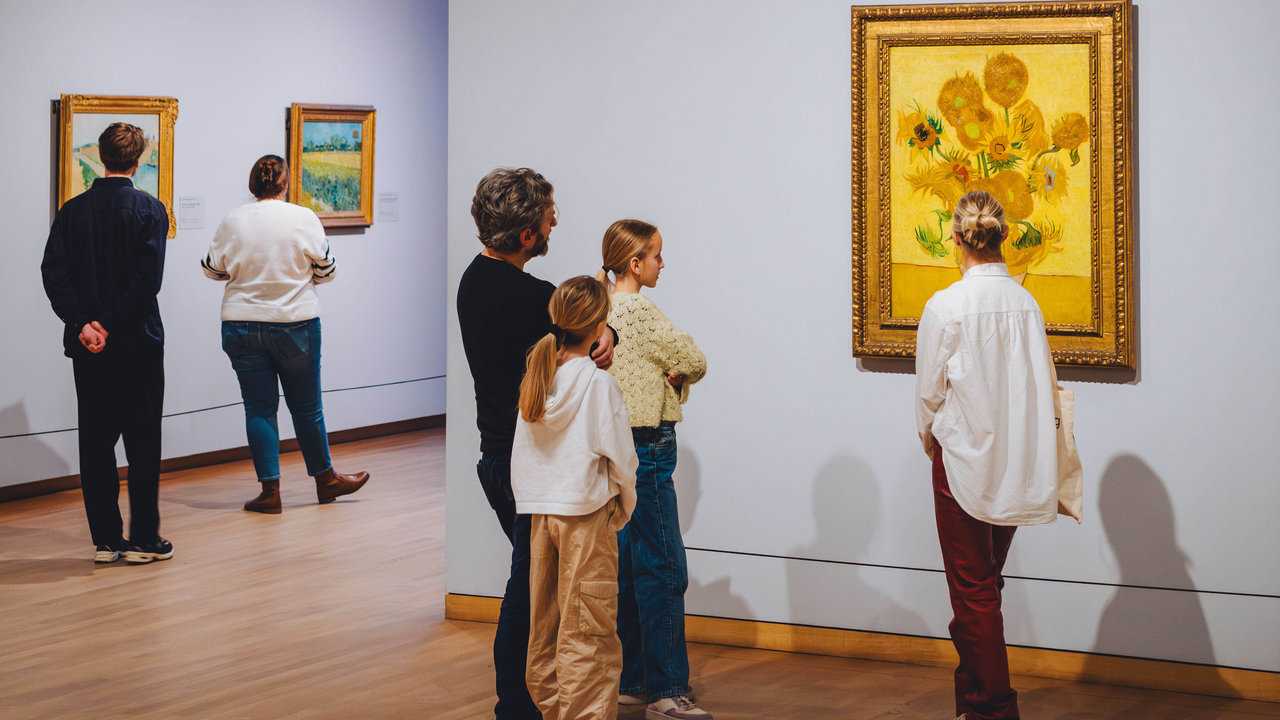
\includegraphics[width=0.5\textwidth]{vangogh_museum.jpg}\label{fig:vangogh}
    \caption{Van Gogh Museum}
\end{figure}

\subsection{De Jordaan}
\url{https://nl.wikipedia.org/wiki/Jordaan_(Amsterdam)}\\
Leuke wijk met veel grachten en smalle straatjes, bevat ook veel leuke winkeltjes en cafeetjes.

\begin{figure}[h]
    \centering
    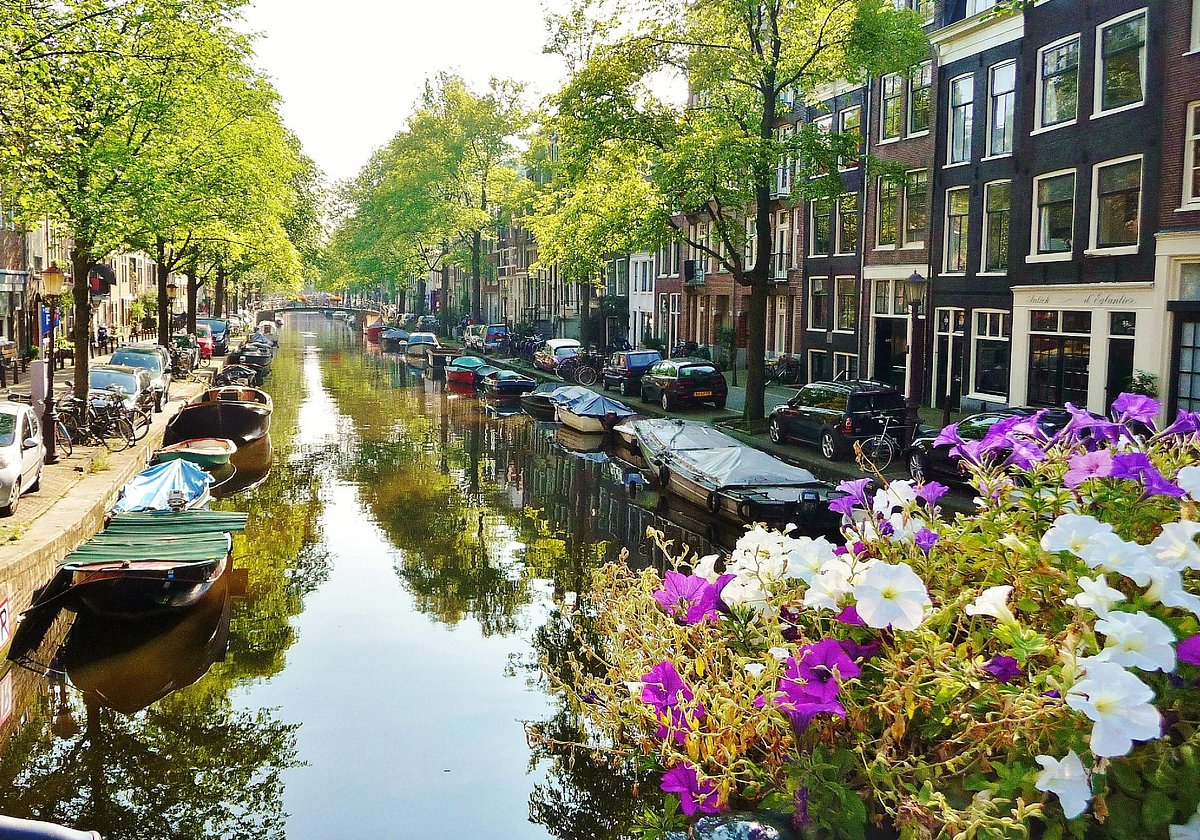
\includegraphics[width=0.5\textwidth]{jordaan-amsterdam.jpg}\label{fig:jordaan}
    \caption{Sfeerbeeld van de Jordaan}
\end{figure}

\subsection{De Wallen}
\url{https://nl.wikipedia.org/wiki/De_Wallen}\\
De meest populaire gratis openluchtattractie van Amsterdam, 
maar ondanks het louche imago is het ook een historische buurt met veel bezienswaardigheden.
Lange kronkelende keienstraatjes, en een 14de eeuwse Gotische kerk.
Ook zijn er veel klassieke restaurantjes en gezellige café's.
's Nachts te bezoeken om de authentieke sfeer te ervaren.

\begin{figure}[h]
    \centering
    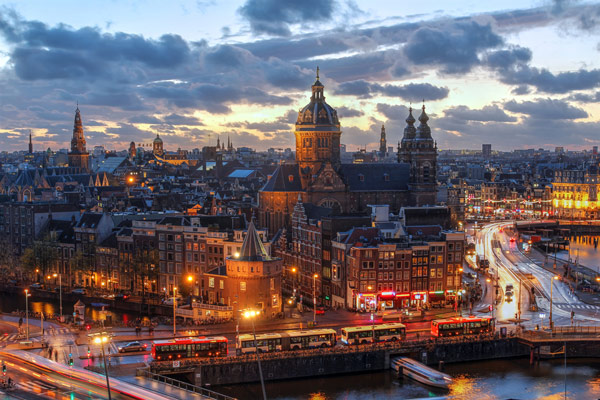
\includegraphics[width=0.5\textwidth]{red-light-district-amsterdam.jpg}\label{fig:wallen}
    \caption{De Wallen}
\end{figure}

\subsection{Albert Cuyp Markt}
\url{https://nl.wikipedia.org/wiki/Albert_Cuypmarkt}\\
De grootste dagmarkt van Nederland, met 260 kramen.

\subsection{Vondelpark}
\url{https://nl.wikipedia.org/wiki/Vondelpark}\\
Stadspark, ontworpen in Engelse landschapsstijl in 1865, met een oppervlakte van 47 hectare.
Misschien wel meer iets voor de zomer, maar kan toch leuk zijn om door te wandelen.

\begin{figure}[h]
    \centering
    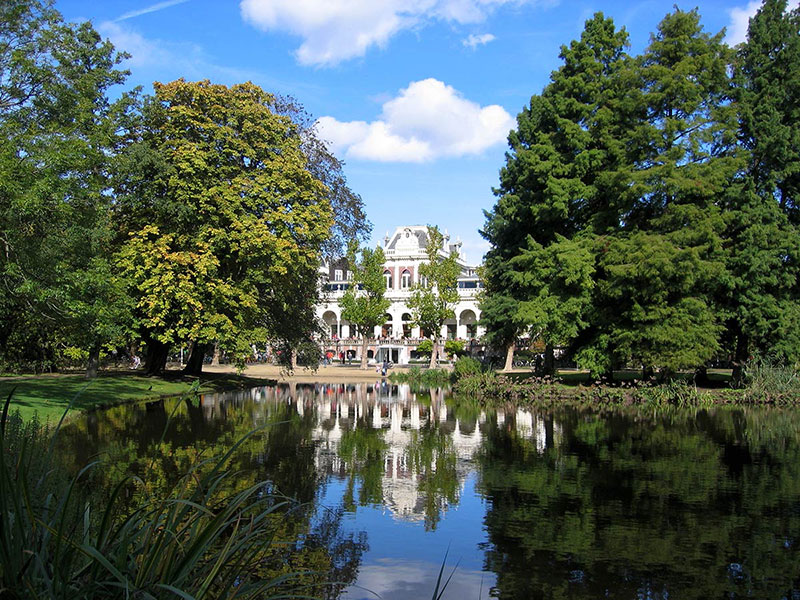
\includegraphics[width=0.5\textwidth]{vondelpark.jpg}\label{fig:vondelpark}
    \caption{Vondelpark}
\end{figure}

\subsection{Wandelen}
Er is zeer veel moois te zien door gewoon rond te wandelen in Amsterdam.

\subsection{Royal Palace Amsterdam}[h]
\url{https://www.paleisamsterdam.nl/}\\
€9,00 per persoon (studentenkorting), maar kan ook leuk zijn om enkel van buitenaf te bekijken\\

\begin{figure}[h]
    \centering
    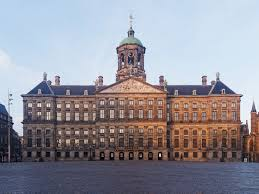
\includegraphics[width=0.5\textwidth]{koninklijk_paleis.jpg}\label{fig:koninklijk_paleis}
    \caption{Royal Palace Amsterdam}
\end{figure}

\subsection{Museum Quarter}
\url{https://nl.wikipedia.org/wiki/Museumplein_(Amsterdam)}\\
Plein waar alle grote musea van Amsterdam liggen, zoals het Rijksmuseum, het Van Gogh Museum en het Stedelijk Museum.

\begin{figure}[h]
    \centering
    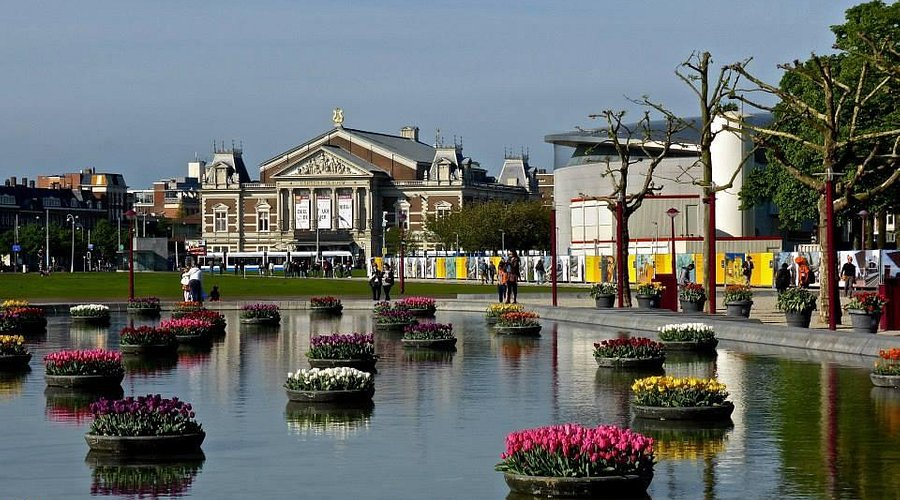
\includegraphics[width=0.5\textwidth]{museumplein.jpg}\label{fig:museumplein}
    \caption{Museumplein}
\end{figure}

\section{Weer}
Ziet er voorlopig goed uit:
\begin{figure}[h]
    \centering
    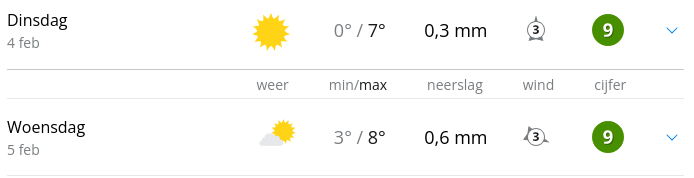
\includegraphics[width=0.5\textwidth]{weerbericht.png}\label{fig:weer}
    \caption{Weersvoorspelling}
\end{figure}

\end{document}